\documentclass[onecolumn,preprintnumbers,amsmath,amssymb]{revtex4}
\usepackage{graphicx}
\usepackage{float}
\usepackage[usenames,dvipsnames]{color}
\begin{document}
\title{Antimatter Freezeout: electron-positron freezeout in early universe}
\author{Cheng Tao Yang${}^a$ and Johann Rafelski${}^a$}
\affiliation{${}^a$Department of Physics, The University of Arizona, Tucson, Arizona 85721, USA}
\date{\today}

%%%%%%%%%%%%%%%%%%%%%%%%%%%%%%%%%%%%%%%%%%%%%%%%%%%%%%%%%%%%%%%%%%
%%%%%%%%%%%%%%%%%%%%%%%%%%%%%%%%%%%%%%%%%%%%%%%%%%%%%%%%%%%%%%%%\propto

%\begin{abstract}
%In this note, we derive the kinetic equation for electron and positron in details. Using the exact Fermi distribution for electron and positron, we obtain the thermal reaction rate per unit time and volume with Fermi-blocking in Eq.~(\ref{Thermal_rate}).
%\end{abstract}
\maketitle

%%%%%%%%%%%%%%%%%%%%%%%%%%%%%%%%%%%%%%%%%%%%%%%%%%%%%%%%%%%%%%%%%
\section{Degenerate Fermi Gas}
In general, the Fermi-Dirac distribution can be written as
\begin{align}
\label{Fermi_exact}
f&=\frac{1}{e^{(E-\tilde{\mu})/T}+1}=\frac{1}{2}\bigg[1-\tanh{\left(\frac{E-\tilde{\mu}_e}{2T}\right)}\bigg],
\end{align}
where the general chemical potential $\tilde\mu$ is given by
\begin{align}
\tilde\mu_e=\pm\mu_e+T\ln\Upsilon_e,
\end{align}
where $"+"$ for particle and $"-"$ for antiparticle. In order to understand the meaning of the parameters $\Upsilon$ and $\mu$, let we consider the first law of thermodynamics. We have
\begin{align}
dE&=-PdV+TdS+{\mu_N}dN+{\mu_{\bar{N}}}d{\bar{N}}
\\&=-PdV+TdS+{\mu}(dN-d{\bar{N}})+T\ln{\Upsilon}(dN+d{\bar{N}})
\end{align}
therefore, we see that the $\mu$ is the energy required to change the difference between particles and antiparticles, and the $T\ln\Upsilon$ is the energy required to change the total number of particle and antiparticle, and the $\Upsilon$ is the parameter to adjust the energy.

In the extreme limit $T\rightarrow0$, the Fermi-Dirac distribution becomes very simple: a state is either filled or empty. We have
\begin{align}
f_e&=\frac{1}{e^{(E-\tilde{\mu})/T}+1}=\left\{\begin{array}{c}1,\,\,\,\mathrm{for}\,\,\,{E}<\tilde{\mu}_e \\0,\,\,\,\mathrm{for}\,\,\, {E}>\tilde{\mu}_e\end{array}\right.
\end{align}
The energy of the last filled state is called the Fermi energy and is denoted as $E_F$. Mathematically, it is the value of the chemical potential at $T=0$, $\tilde\mu(T = 0)=E_F$. In Fig.(\ref{Electron_001}) we plot the Fermi-distribution of electron as a function of energy where the parameters are given by $T=0.012\,\mathrm{MeV}$, $\Upsilon_e=\Upsilon_{\bar e}=1$, and chemical potential $\mu_e=m_e-\delta$ with $\delta=0.05\,\mathrm{MeV}$.
%~~~~~~~Figure~~~~~~~~~~~~~~~~~~~~~~~~~~~~~~~~~~~~~~~~~~~~~~~~~~~~~~~~~~~~~~~~~~~~~~~~~~~~~~~~~~~~~
\begin{figure}[h]
\begin{center}
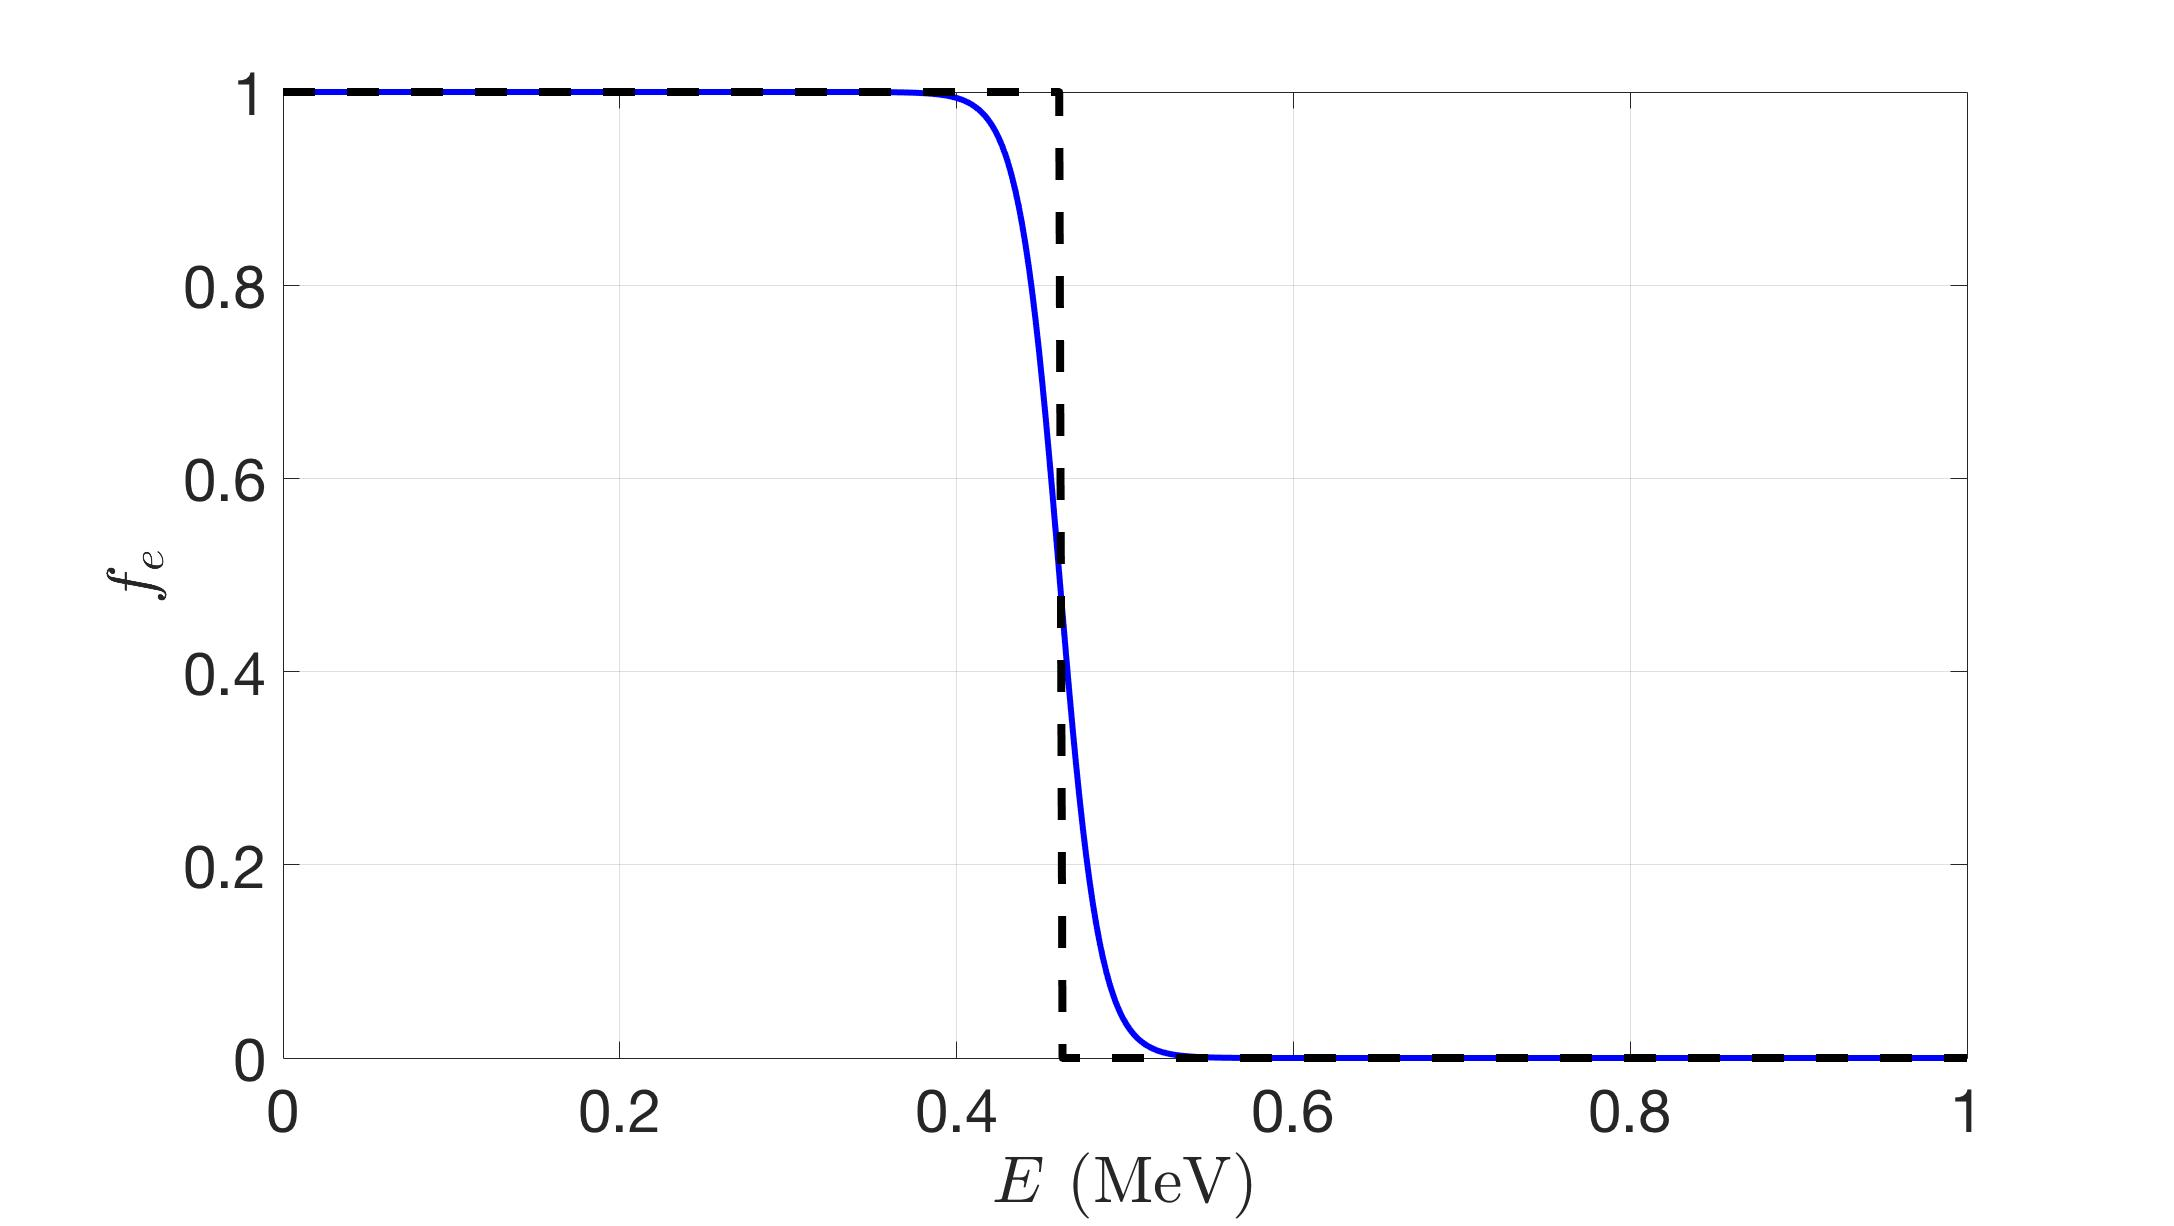
\includegraphics[width=0.9\textwidth]{./plot/Electron_distribution001}
\caption{The Fermi-distribution of electron as a function of energy where the parameters are given by $T=0.012\,\mathrm{MeV}$, $\Upsilon_e=\Upsilon_{\bar e}=1$, and chemical potential $\mu_e=m_e-\delta$ with $\delta=0.05\,\mathrm{MeV}$.}
\label{Electron_001}
\end{center}
\end{figure}
%~~~~~~~~~~~~~~~~~~~~~~~~~~~~~~~~~~~~~~~~~~~~~~~~~~~~~~~~~~~~~~~~~~~~~~~~~~~~~~~~~~~~~~~~~~~~~~~

%%%%%%%%%%%%%%%%%%%%%%%%%%%%%%%%%%%%%%%%%%%%%%%%%%%%%%%%%%%%%%%%%
\section{A new form of Fermi-distribution} 
In general, using the step-function the Fermi-distribution can be written as
\begin{align}
\label{Fermi_distribution}
f_e(E)&=f_{cold}+f_\delta(E)+f_\epsilon(E)\\
&=\Theta(E_F-E)+\frac{1}{2}\frac{(E-E_F)}{|E-E_F|}\,e^{-|E-E_F|/T}+\frac{1}{2}e^{-|E-E_F|/T}\,\tanh\bigg[\frac{E-E_F}{2T}\bigg],
\end{align}
where the $f_{cold}=\Theta(E_F-E)$ represents the cold Fermi gas and the Fermi energy is given by
\begin{align}
E_F=\mu_e+T\ln\Upsilon_e=\left(m_e-\epsilon\right)+T\ln\Upsilon_e.
\end{align}
Then we have
\begin{align}
\left(E_F-m_e\right)=-\epsilon+T\ln\Upsilon_e\left\{\begin{array}{c}>0 \\=0 \\<0\end{array}\right.
\end{align}
In Fig.(\ref{Fermi_Step}) we plot the Fermi-distribution Eq.(\ref{Fermi_exact}) (blue solid line) and Eq.(\ref{Fermi_distribution}) (red dash line) as a function of energy where the parameters are given by $T=0.012\,\mathrm{MeV}$, $\Upsilon_e=\Upsilon_{\bar e}=1$, and chemical potential $\mu_e=m_e-\delta$ with $\delta=0.05\,\mathrm{MeV}$.
%~~~~~~~Figure~~~~~~~~~~~~~~~~~~~~~~~~~~~~~~~~~~~~~~~~~~~~~~~~~~~~~~~~~~~~~~~~~~~~~~~~~~~~~~~~~~~~~
\begin{figure}[h]
\begin{center}
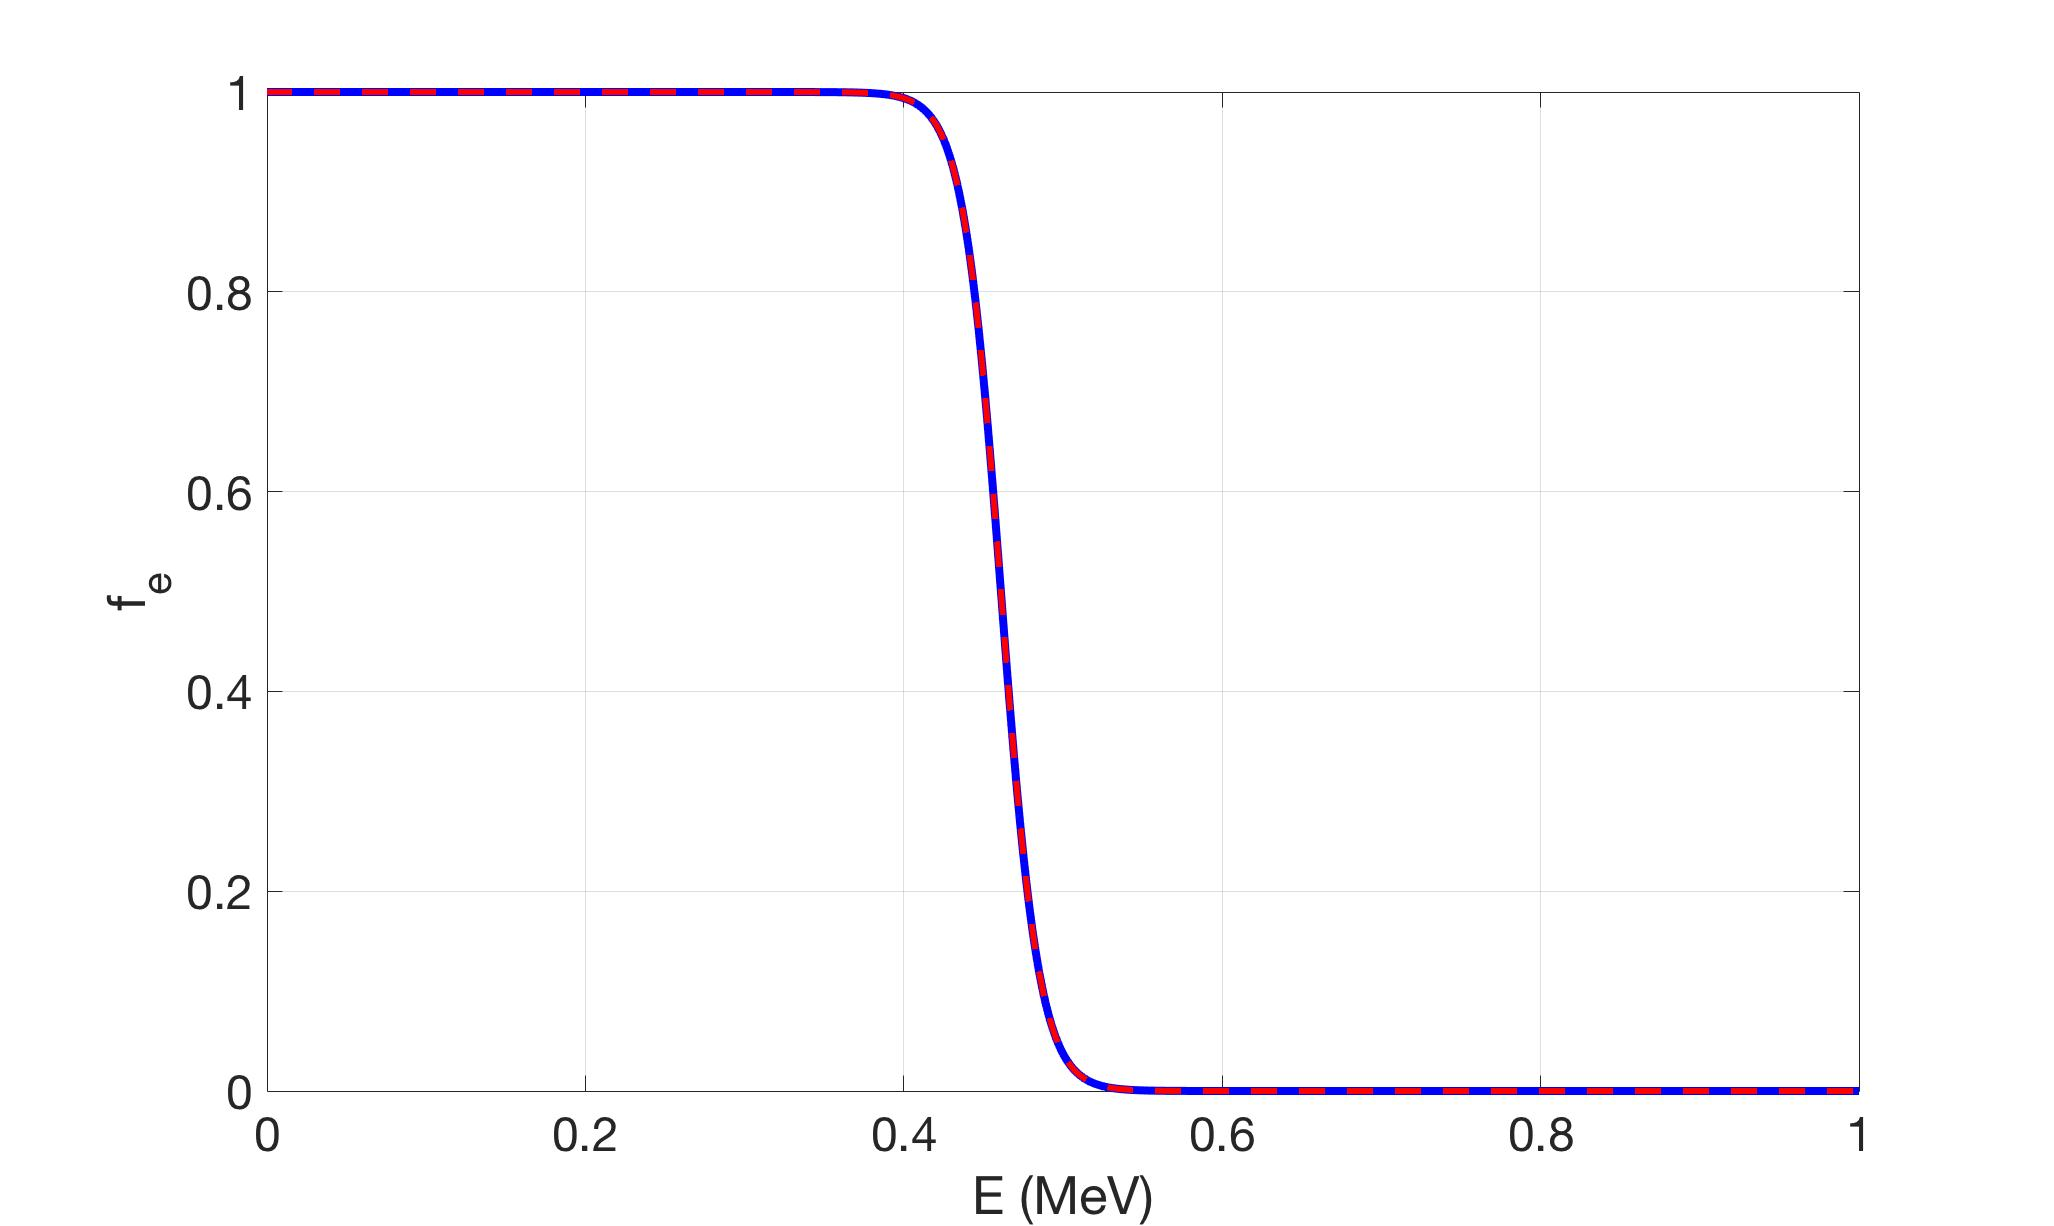
\includegraphics[width=0.9\textwidth]{./plot/Fermi_step}
\caption{We plot the Fermi-distribution Eq.(\ref{Fermi_exact})(blue solid line) and Eq.(\ref{Fermi_distribution})(red dash line) as a function of energy where the parameters are given by $T=0.012\,\mathrm{MeV}$, $\Upsilon_e=\Upsilon_{\bar e}=1$, and chemical potential $\mu_e=m_e-\delta$ with $\delta=0.05\,\mathrm{MeV}$.}
\label{Fermi_Step}
\end{center}
\end{figure}
%~~~~~~~~~~~~~~~~~~~~~~~~~~~~~~~~~~~~~~~~~~~~~~~~~~~~~~~~~~~~~~~~~~~~~~~~~~~~~~~~~~~~~~~~~~~~~~~~~

In Fig. (\ref{Fermi_Checking}) and Fig(\ref{Fermi_Checking2}) we plot the Fermi-distribution Eq.(\ref{Fermi_exact}) (solid line) and Eq.(\ref{Fermi_distribution}) (dash line) as a function of energy with different parameters. On the left hand side we plot the Fermi distribution with different chemical potential: $\tilde\mu=0, 0.111, 0.461\, \mathrm{MeV}$ at temperature $T=0.012\,\mathrm{MeV}$. On the right hand side we have Fermi distribution with different temperature $T=0.511, 0.0511, 0.012\,\mathrm{MeV}$ with chemical potential $\tilde\mu=0.461\,\mathrm{MeV}$.
%~~~~~~~Figure~~~~~~~~~~~~~~~~~~~~~~~~~~~~~~~~~~~~~~~~~~~~~~~~~~~~~~~~~~~~~~~~~~~~~~~~~~~~~~~~~~~~~
\begin{figure}[h]
\begin{center}
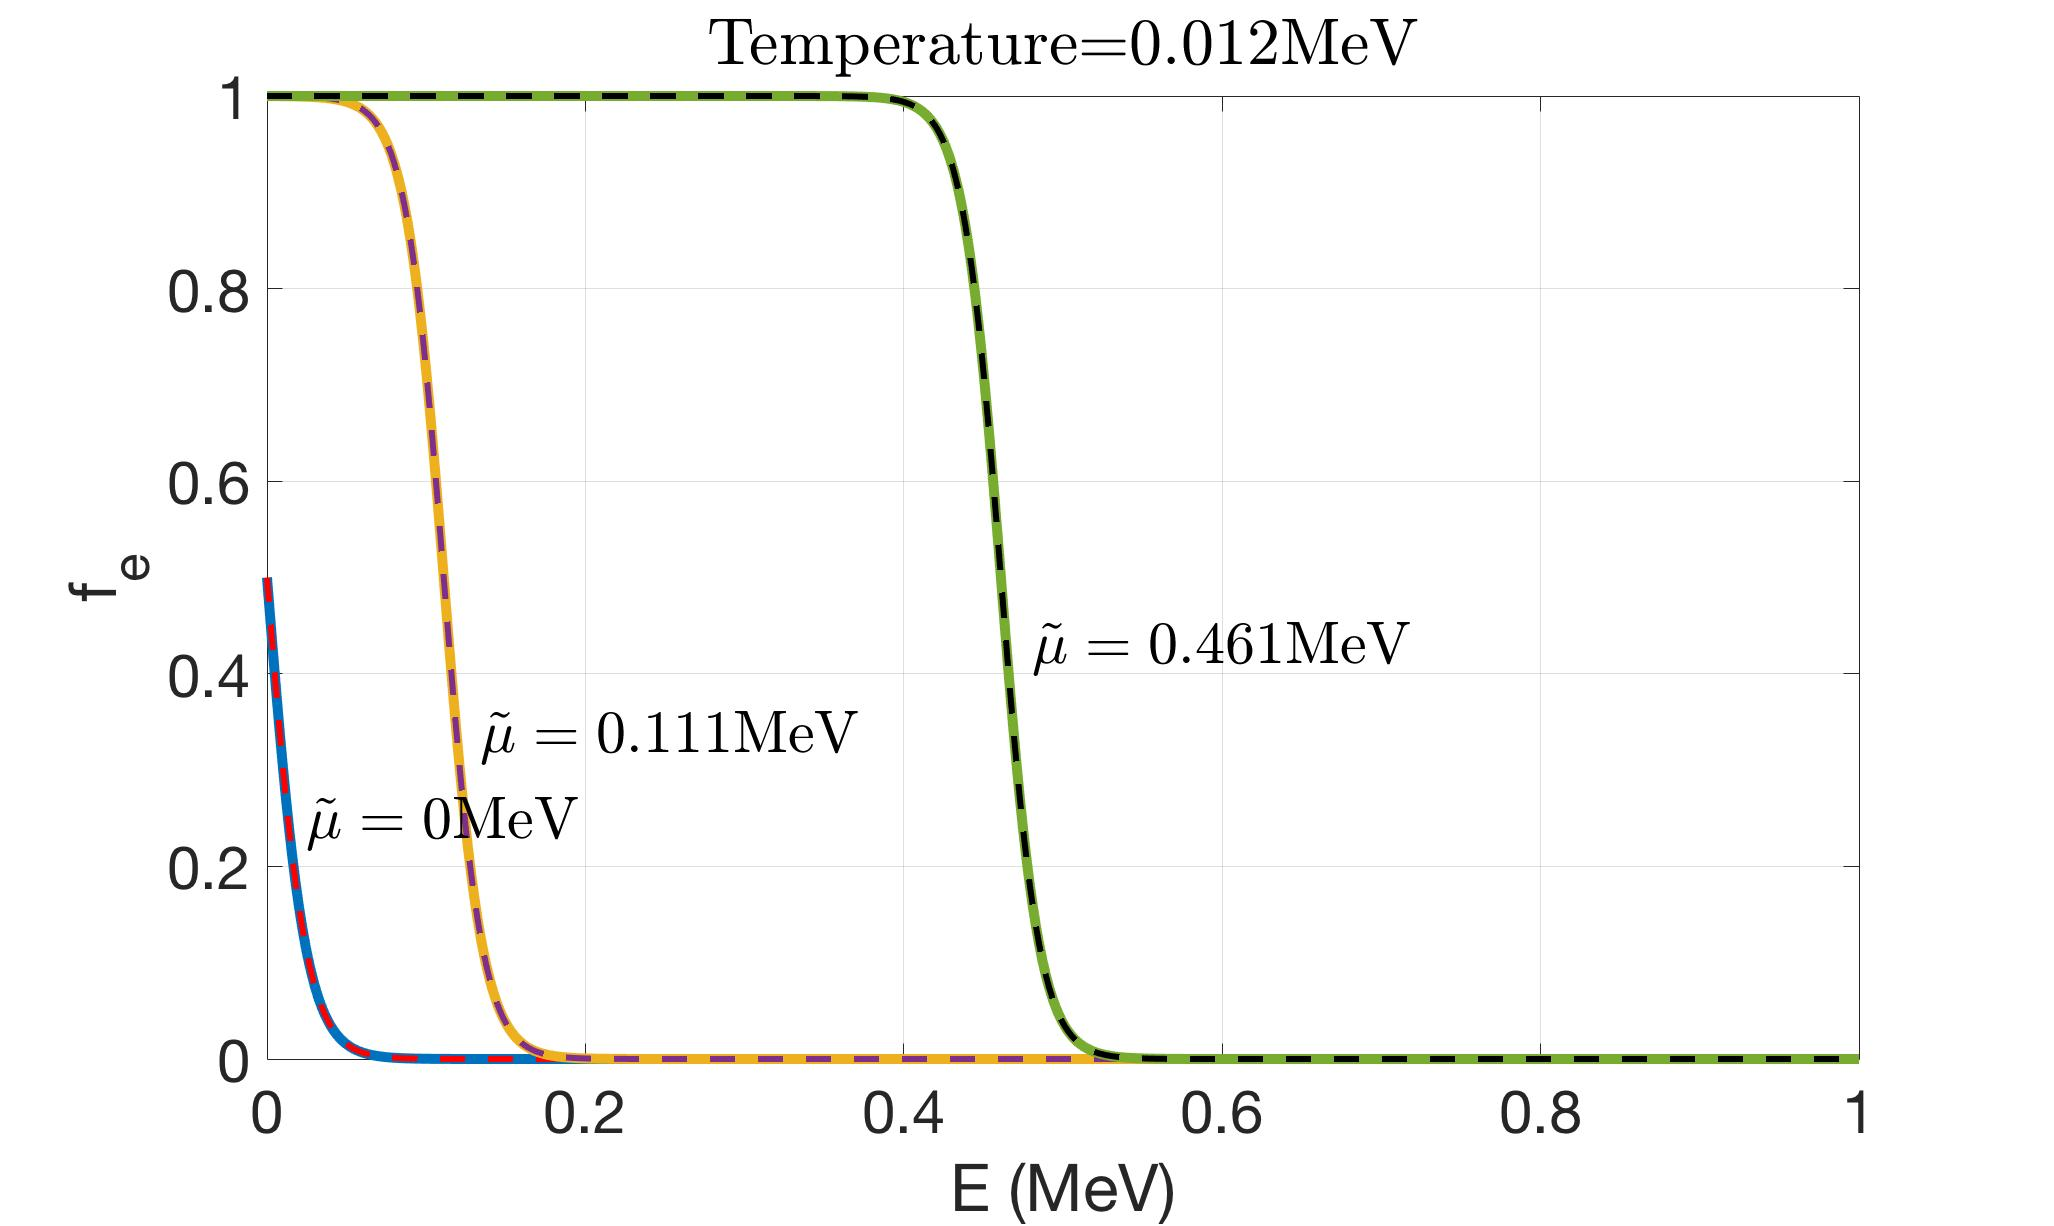
\includegraphics[width=0.45\textwidth]{./plot/Fermi_Chemical_Potential}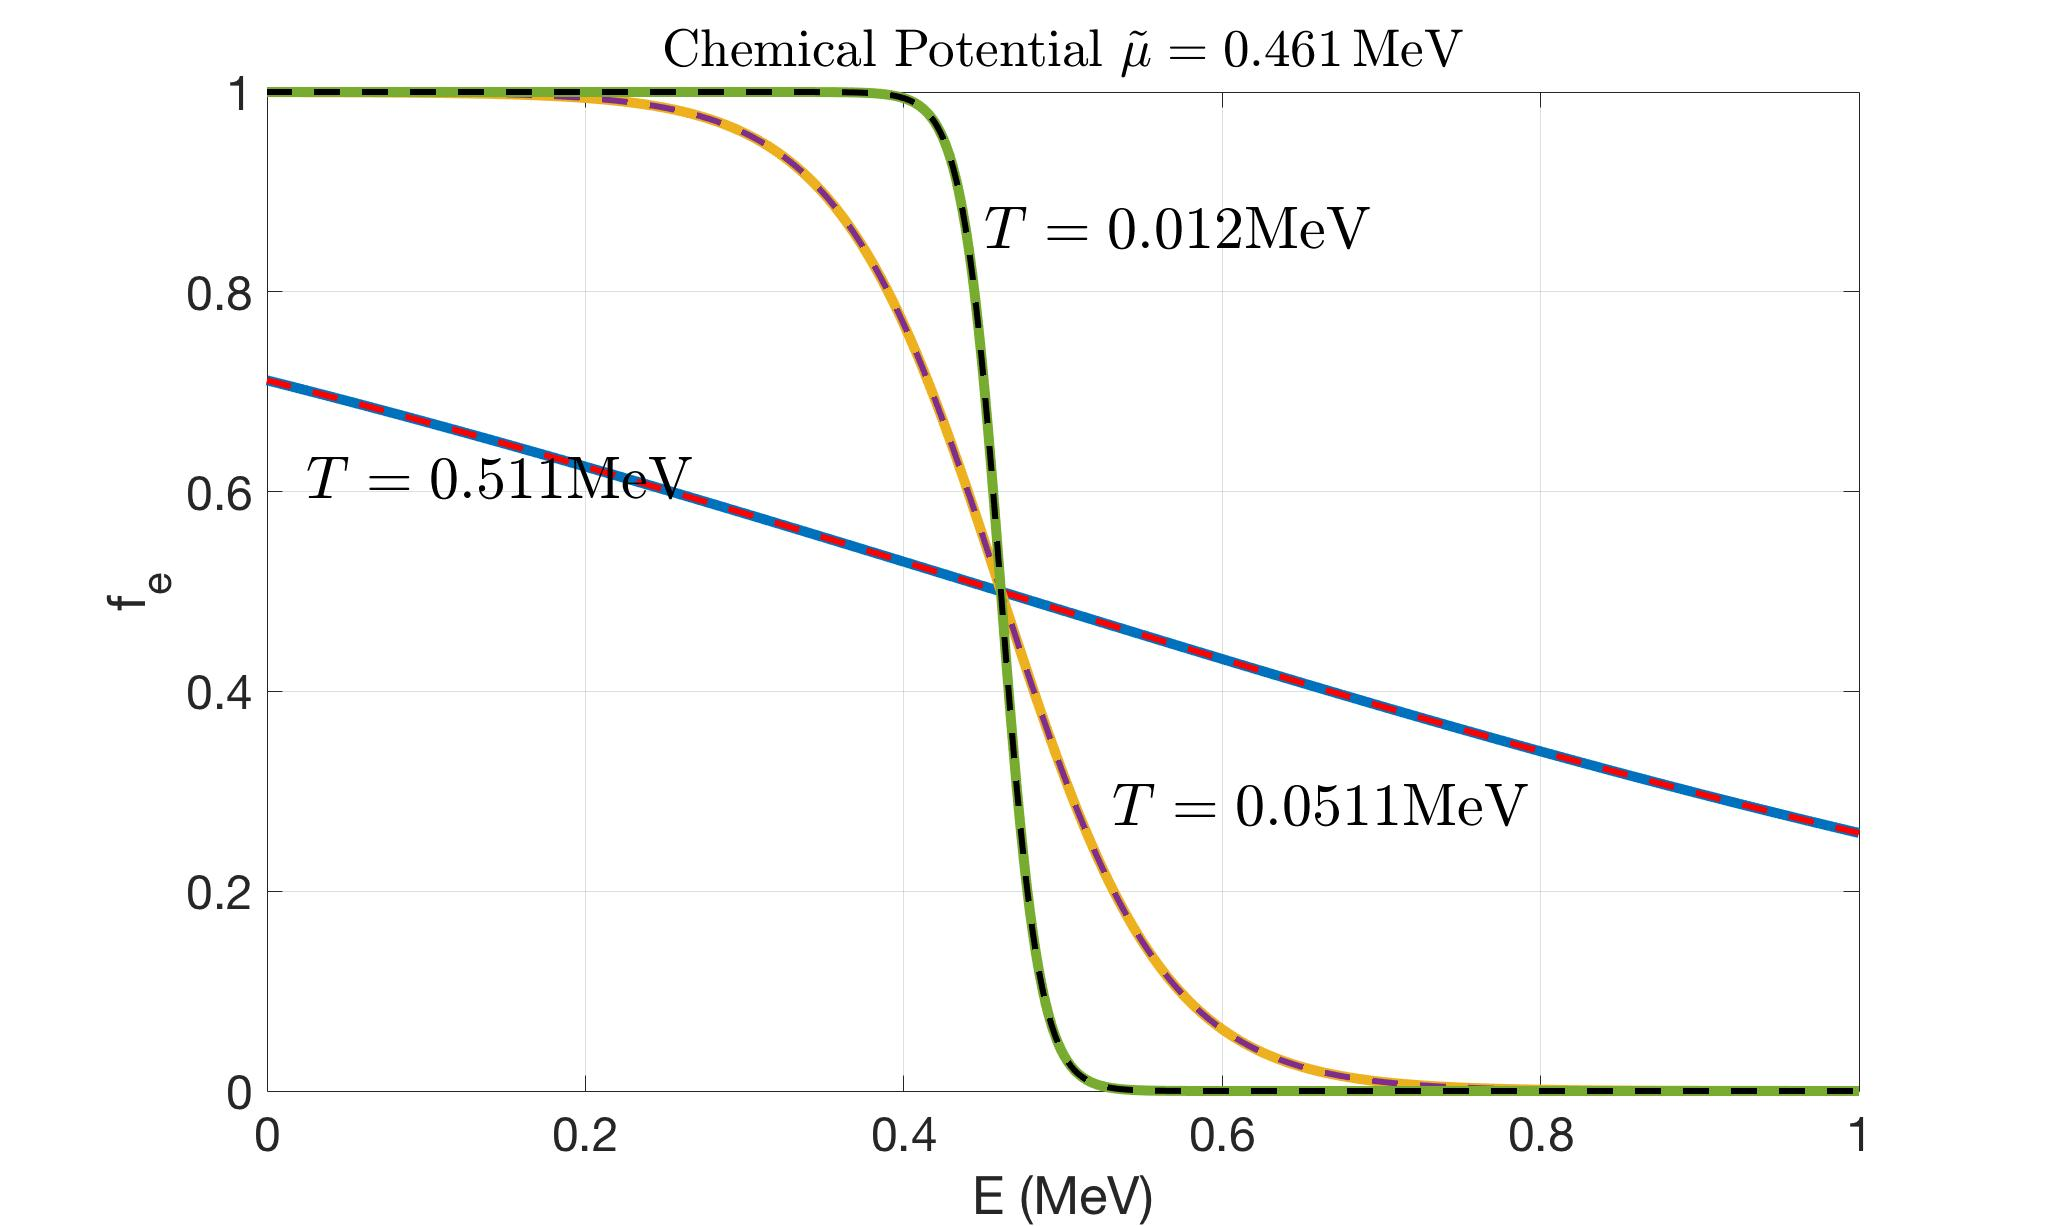
\includegraphics[width=0.45\textwidth]{./plot/FermI_Temperature}
\caption{We plot the Fermi-distribution Eq.(\ref{Fermi_exact}) (solid line) and Eq.(\ref{Fermi_distribution}) (dash line) as a function of energy with different parameters. On the left hand side: the Fermi distribution with different chemical potential: $\tilde\mu=0, 0.111, 0.461\, \mathrm{MeV}$ at temperature $T=0.012\,\mathrm{MeV}$. On the right hand side: the Fermi distribution with different temperature $T=0.511, 0.0511, 0.012\,\mathrm{MeV}$ with chemical potential $\tilde\mu=0.461\,\mathrm{MeV}$.}
\label{Fermi_Checking}
\end{center}
\end{figure}
%~~~~~~~~~~~~~~~~~~~~~~~~~~~~~~~~~~~~~~~~~~~~~~~~~~~~~~~~~~~~~~~~~~~~~~~~~~~~~~~~~~~~~~~~~~~~~~~~~
%~~~~~~~Figure~~~~~~~~~~~~~~~~~~~~~~~~~~~~~~~~~~~~~~~~~~~~~~~~~~~~~~~~~~~~~~~~~~~~~~~~~~~~~~~~~~~~~
\begin{figure}[h]
\begin{center}
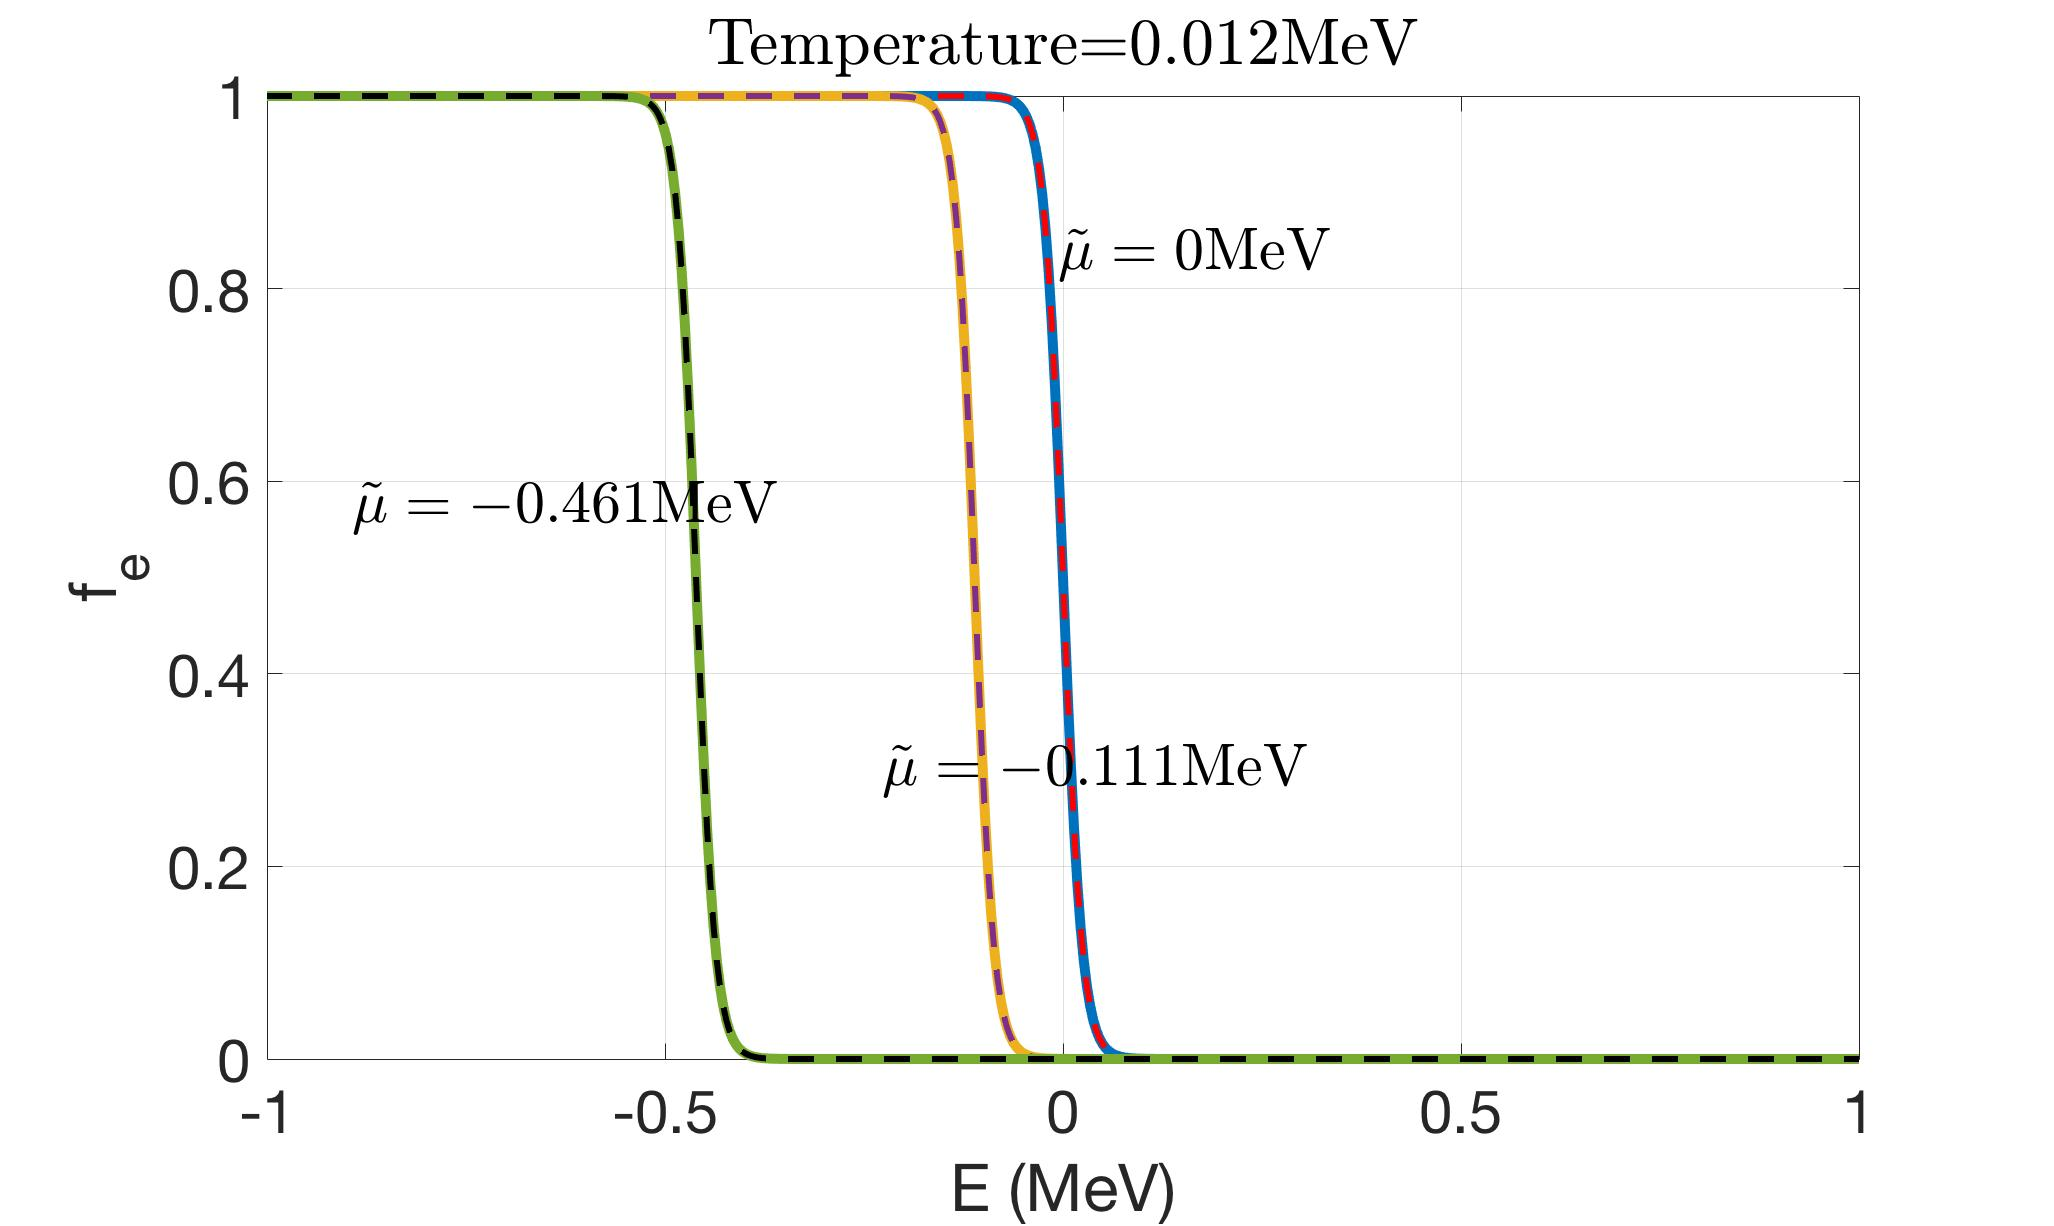
\includegraphics[width=0.45\textwidth]{./plot/Fermi_Chemical_negative}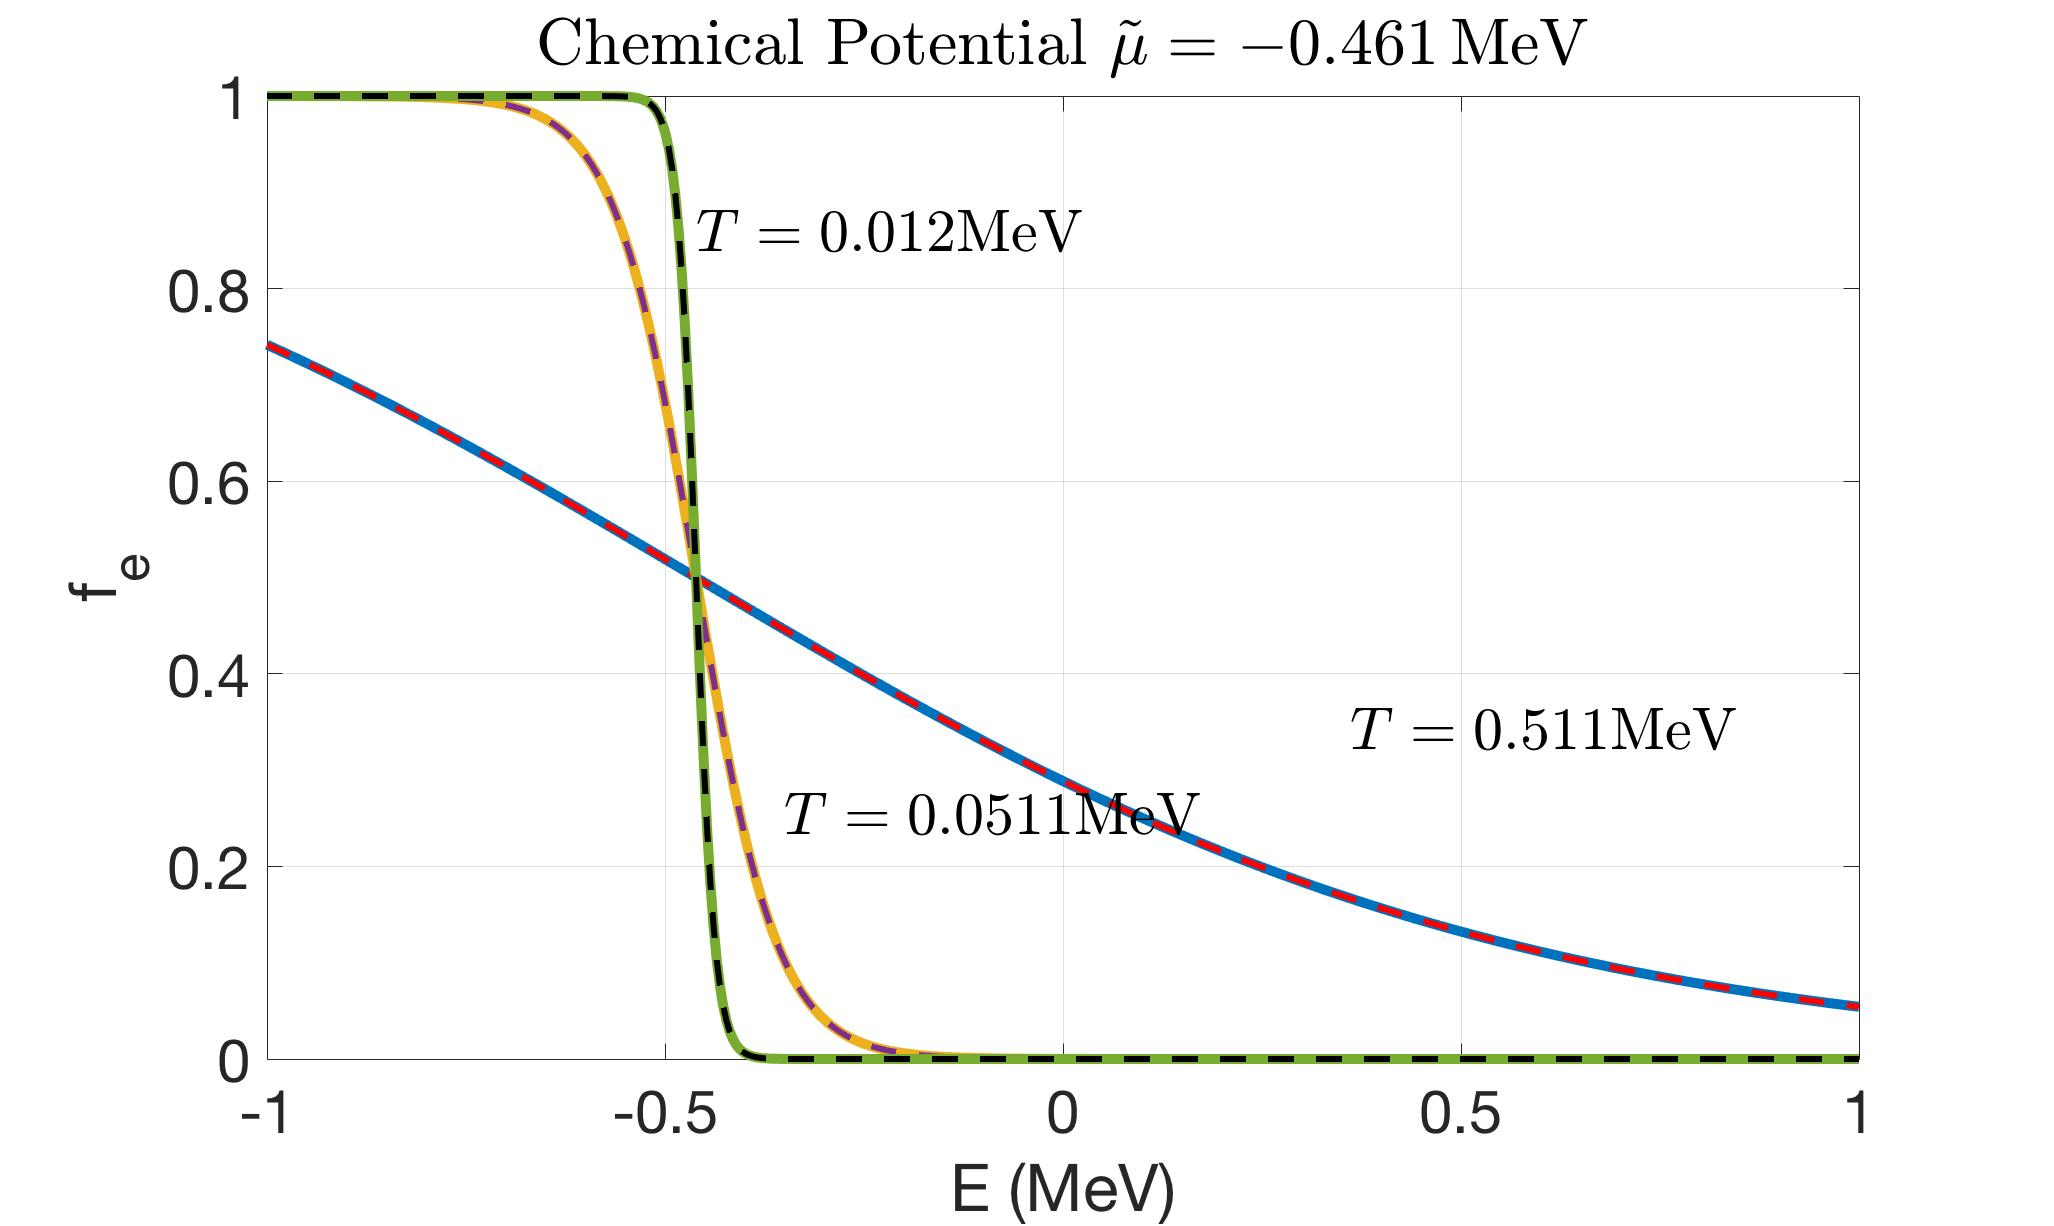
\includegraphics[width=0.45\textwidth]{./plot/Fermi_Temperature_negative}
\caption{We plot the Fermi-distribution Eq.(\ref{Fermi_exact}) (solid line) and Eq.(\ref{Fermi_distribution}) (dash line) as a function of energy:$-1\,\mathrm{MeV}\leqslant E\leqslant1\,\mathrm{MeV}$ with different parameters. On the left hand side: the Fermi distribution with different chemical potential: $\tilde\mu=0, -0.111, -0.461\, \mathrm{MeV}$ at temperature $T=0.012\,\mathrm{MeV}$. On the right hand side: the Fermi distribution with different temperature $T=0.511, 0.0511, 0.012\,\mathrm{MeV}$ with chemical potential $\tilde\mu=-0.461\,\mathrm{MeV}$.}
\label{Fermi_Checking2}
\end{center}
\end{figure}
%~~~~~~~~~~~~~~~~~~~~~~~~~~~~~~~~~~~~~~~~~~~~~~~~~~~~~~~~~~~~~~~~~~~~~~~~~~~~~~~~~~~~~~~~~~~~~~~

%%%%%%%%%%%%%%%%%%%%%%%%%%%%%%%%%%%%%%%%%%%%%%%%%%%%%%%%%%%%%%

In general the Fermi-distribution is given by
\begin{align}
f_e=f_{cold} +f_\delta+f_\epsilon.
\end{align}
For any given function $g(E)$, then the correspond physical quantity can be written as
\begin{align}
A\equiv\int^{\infty}_{m_e}dE\,g(E)\,f_e(E)=\int^{\infty}_{m_e}dE\,g(E)\bigg[f_{cold} +f_\delta+f_\epsilon\bigg].
\end{align}
Integrating by part, the quantity $A$ can be written as
\begin{align}
\label{N_electron}
A=\int^{\infty}_{m_e}dE\,\rho(E)\,f_e(E)=A_{cold}+\int^{\infty}_{m_e}\,dE\left(g(E)\,f_\delta(E)-g^\prime(E)\,f^{(2)}_\delta(E)\right)+\left.g(E)\,f^{(2)}_\delta\right|_{surface},
\end{align}
where $g^\prime(e)=dg(E)/dE$ and the function $f^{(2)}_\delta(E)$ is defined as
\begin{align}
f^{(2)}_\delta(E)=\int^E_{m_e}dE^\prime\,f_\epsilon(E^\prime).
\end{align}
%%%%%%%%%%%%%%%%%%%%%%%%%%%%%%%%%%%%%%%%%%%%%%%%%%%%%%%%%%%%%%%%%
%%%%%%%%%%%%%%%%%%%%%%%%%%%%%%%%%%%%%%%%%%%%%%%%%%%%%%%%%%%%%%%%%
\subsection{The Influence of $f_{\delta}(E)$}
In our case, from the Fermi-distribution Eq.(\ref{Fermi_distribution}) the function $f_\delta(E)$ is given by:
\begin{align}
f_{\delta}(E)&=\frac{1}{2}\frac{(E-E_F)}{|E-E_F|}\,e^{-|E-E_F|/T},
\end{align}
In Fig.(\ref{f_delta_graph}) we plot the function $f_{\delta\mathcal{P}}(E)$ as a function of energy $E$ at temperature $T=0.012\,\mathrm{MeV}$ with difference Fermi-energy $E_F=0.111\,\mathrm{MeV},0.461\,\mathrm{MeV},$. We found that the function $f_\delta(E)$ has positive and negative peaks at $E=E_F$.  %~~~~~~~Figure~~~~~~~~~~~~~~~~~~~~~~~~~~~~~~~~~~~~~~~~~~~~~~~~~~~~~~~~~~~~~~~~~~~~~~~~~~~~~~~~~~~~~
\begin{figure}[t]
\begin{center}
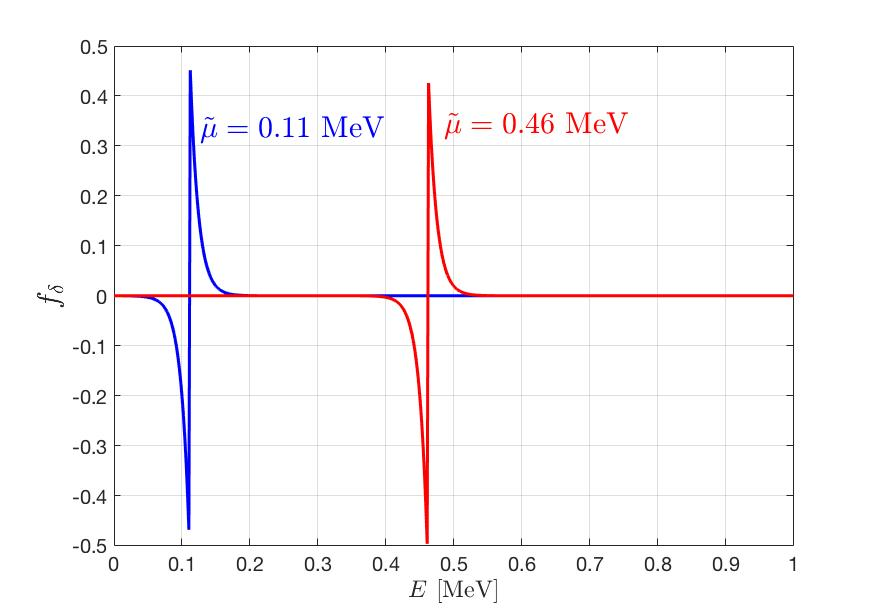
\includegraphics[width=0.9\textwidth]{./plot/f_delta}
\caption{We plot the function $f_\delta$ as a function of energy $E$ at temperature $T=0.012\,\mathrm{MeV}$ with difference Ferni-energy $E_F=0.111\,\mathrm{MeV}(blue line),0.461\,\mathrm{MeV}(red line),$. We found that the function has positive and negative peaks at  $E=E_F$. }
\label{f_delta_graph}
\end{center}
\end{figure}
%~~~~~~~~~~~~~~~~~~~~~~~~~~~~~~~~~~~~~~~~~~~~~~~~~~~~~~~~~~~~~~~~~~~~~~~~~~~~~~~~~~~~~~~~~~~~~~~~

In general, for any given function $g(E)$ the integral for $f_\delta(E)$ is given by
\begin{align}
\label{Integral001}
\int^{\infty}_{m_e}\,dE\,g(E)\,f_\delta(E)=\int^\infty_{m_e}\,dE\,g(E)\,\left[\,\frac{1}{2}\frac{(E-E_F)}{|E-E_F|}\,e^{-|E-E_F|/T}\,\right].
\end{align}
It is convenient to introduce the dimensionless variable as below:
\begin{align}
x\equiv\left(\frac{E-E_F}{T}\right),
\end{align}
then the dimensionless integral can be written as
\begin{align}
\int^\infty_{x_0}\,dx\,g(x)\,\left[\,\frac{1}{2}\frac{x}{|x|}\,e^{-|x|}\,\right],
\end{align}
where the parameter $x_0=(m_e-E_F)/T$. To calculate the integral we need to consider the case as follows
\begin{itemize}
  \item Considering $x_0>0$, i.e., $m_e>E_F$. We have
  \begin{align}
  \frac{1}{2}\int^\infty_{x_0}\,dx\,g(x)\frac{x}{|x|}\,e^{-|x|}=\frac{1}{2}\int^{\infty}_{x_0}\,dx\,g(x)\,e^{-x}.
  \end{align}
  In this case, we have the integral with Boltzmann gas distribution.
  \item Considering $x_0<0$, i.e., $m_e<E_F$. We obtain
  \begin{align}
   \frac{1}{2}\int^\infty_{-|x_0|}dx\,g(x)\frac{x}{|x|}\,e^{-|x|}&=\frac{1}{2}\left[\left(\int_0^{|x_0|}dx\,g(x)\,\frac{x}{|x|}\,e^{-|x|}+\int^\infty_{|x_0|}dx\,g(x)\,\frac{x}{|x|}\,e^{-|x|}\right)+\int^0_{-|x_0|}dx\,g(x)\,\frac{x}{|x|}\,e^{-|x|}\right]\notag\\
   &=\frac{1}{2}\left[\int_{-|x_0|}^{|x_0|}dx\,g(x)\,\frac{x}{|x|}\,e^{-|x|}+\int^\infty_{|x_0|}dx\,g(x)\,\frac{x}{|x|}\,e^{-|x|}\right]\notag\\
   &=\frac{1}{2}\left[\int_{0}^{|x_0|}dx\,\left(g(x)+g(-x)\right)\,e^{-x}+\int^\infty_{|x_0|}dx\,g(x)\,e^{-x}\right].
  \end{align}
  In this case the $1st$ integral gives us the correction beside the Boltzmann gas.
\end{itemize}
In summary, the dimensionless integral is given by
\begin{align}
\int^\infty_{x_0}\,dx\,g(x)\,\left(\,\frac{1}{2}\frac{x}{|x|}\,e^{-|x|}\,\right)=\Theta(-x_0)\,\frac{1}{2}\int_{0}^{|x_0|}dx\,\bigg[g(x)+g(-x)\bigg]\,e^{-x}+\frac{1}{2}\int^\infty_{|x_0|}dx\,g(x)\,e^{-x}.
\end{align}
We found that the 1st  integral only exist when the Fermi energy $E_F>m_e$ and given function $g(x)$ is even function. Otherwise we only have the Boltzmann integral.
%%%%%%%%%%%%%%%%%%%%%%%%%%%%%%%%%%%%%%%%%%%%%%%%%%%%%%%%%%%%%%%%%

\subsection{The Influence of $f^{(2)}_\delta(E)$}
On the other hand, from the Fermi-distribution Eq.(\ref{Fermi_distribution}) the function$f^{(2)}_\delta(E)$ is given by
\begin{align}
f^{(2)}_\delta(E)&=\frac{1}{2}\int^{E}_{m_e}\,dE^\prime\,e^{-|E^\prime-E_F|/T}\,\tanh\bigg[\frac{E^\prime-E_F}{2T}\bigg]\notag\\
&=\frac{T}{2}\left[e^{-|E_F-E|/T}-e^{-|E_F-m_e|/T}+2\ln{\left(\frac{1+e^{-|E_F-m_e|/T}}{1+e^{-|E_F-E|/T}}\right)}\right].
\end{align}
In Fig.(\ref{f_delta002_graph}) we plot the function $f_\delta$ as a function of energy $E$ at temperature $T=0.012\,\mathrm{MeV}$ with difference Fermi-energy $E_F=0.4\,\mathrm{MeV},me, 0.6\,\mathrm{MeV}, 0.7\,\mathrm{MeV},0.8\,\mathrm{MeV}$. We found that the function $f^{(2)}_\delta(E)$ has peaks at $E=E_F$.  Also, in Fig.(\ref{f_delta_checking_graph}) we plot the function$f^{(2)}_\delta$ as a function $E_f$ and we found that the function $f^{(2)}_\delta(E)$ also has peaks when the $E_F=m_e$.

In general, for a given function $g(E)$ the integral for $f_\delta^{(2)}(E)$ is given by
\begin{align}
\label{Integral002}
\int^\infty_{m_e}dE\,g^\prime(E)\,f^{(2)}_\delta(E)=\int^\infty_{m_e}dE\,g^\prime(E)\frac{T}{2}\bigg[e^{-|E_F-E|/T}-e^{|E_F-m_e|/T}+2\ln\left(\frac{1+e^{-|E_F-m_e|/T}}{1+e^{|E_F-E|/T}}\right)\bigg],
\end{align}
where $g^\prime(E)=dg(E)/dE$. It is also convenient to introduce the dimensionless variable as follows
\begin{align}
x\equiv\frac{E-E_F}{T},
\end{align}
then the dimensionless integral can be written as
\begin{align}
\frac{1}{2}\int^\infty_{x_0}dx\,g^\prime(x)\bigg[e^{-|x|}-e^{-|x_0|}+2\ln\left(\frac{1+e^{-|x_0|}}{1+e^{-|x|}}\right)\bigg],
\end{align}
where the parameter $x_0=(m_e-E_F)/T$. To calculate the integral we need to consider the case as follows
\begin{itemize}
  \item For the case $x_0>0$, i.e., $m_e>E_F$. We obtain
  \begin{align}
  &\frac{1}{2}\int^\infty_{x_0}dx\,g^\prime(x)\bigg[e^{-|x|}-e^{-|x_0|}+2\ln\left(\frac{1+e^{-|x_0|}}{1+e^{-|x|}}\right)\bigg]=\frac{1}{2}\int^\infty_{x_0}dx\,g^\prime(x)\bigg[e^{-x}-e^{-x_0}+2\ln\left(\frac{1+e^{-x_0}}{1+e^{-x}}\right)\bigg]
  \end{align}
  \item For the case $x_0<0$, i.e., $m_e<E_F$. We have
  \begin{align}
   &\frac{1}{2}\int^\infty_{-|x_0|}dx\,g^\prime(x)\bigg[e^{-|x|}-e^{-|x_0|}+2\ln\left(\frac{1+e^{-|x_0|}}{1+e^{-x}}\right)\bigg]\notag\\
   &=\frac{1}{2}\bigg[\left(\int^{|x_0|}_0dx\left(g^\prime(x)+g^\prime(-x)\right)\,e^{-x})+\int^\infty_{|x_0|}dx\,g^\prime(x)\,e^{-|x|}\right)+\left(\int^{|x_0|}_0dx\left(g^\prime(x)+g^\prime(-x)\right)\,e^{-|x_0|}+\int^\infty_{|x_0|}dx\,g^\prime(x)\,e^{-|x_0|}\right)\notag\\
   &+\left(\int^{|x_0|}_0dx\left(g^\prime(x)+g^\prime(-x)\right)\,2\ln\left(\frac{1+e^{-|x_0|}}{1+e^{-x}}\right)+\int^\infty_{|x_0|}dxg^\prime(x)\,2\ln\left(\frac{1+e^{-|x_0|}}{1+e^{-x}}\right)\right)\bigg]
  \end{align}
\end{itemize}
%~~~~~~~Figure~~~~~~~~~~~~~~~~~~~~~~~~~~~~~~~~~~~~~~~~~~~~~~~~~~~~~~~~~~~~~~~~~~~~~~~~~~~~~~~~~~~~~
\begin{figure}[t]
\begin{center}
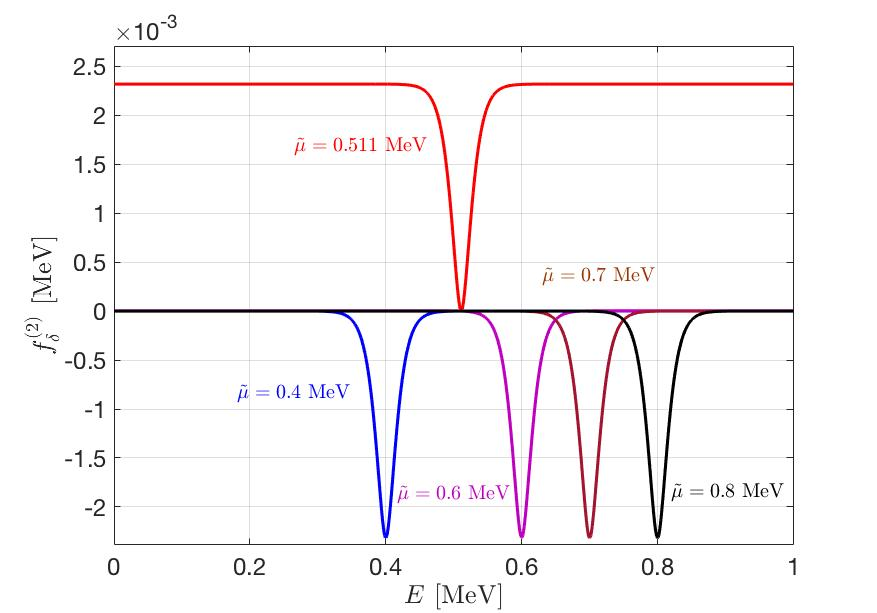
\includegraphics[width=0.9\textwidth]{./plot/f_delta002}
\caption{We plot the function $f^{(2)}_\delta$ as a function of energy $E$ at temperature $T=0.012\,\mathrm{MeV}$ with Fermi-energy around the $m_e$. We have $E_F=0.4\,\mathrm{MeV\,(blue)}, m_e\mathrm{(red)}, 0.6\mathrm{MeV\,(purple)}, 0.7\mathrm{MeV\,(brown)}, 0.8\,\mathrm{MeV\,(black)}$. We found that the function $f^{(2)}_\delta(E)$ has peaks when the energy  $E=E_F$. }
\label{f_delta002_graph}
\end{center}
\end{figure}
%~~~~~~~~~~~~~~~~~~~~~~~~~~~~~~~~~~~~~~~~~~~~~~~~~~~~~~~~~~~~~~~~~~~~~~~~~~~~~~~~~~~~~~~~~~~~~~~~~
%~~~~~~~Figure~~~~~~~~~~~~~~~~~~~~~~~~~~~~~~~~~~~~~~~~~~~~~~~~~~~~~~~~~~~~~~~~~~~~~~~~~~~~~~~~~~~~~
\begin{figure}[h]
\begin{center}
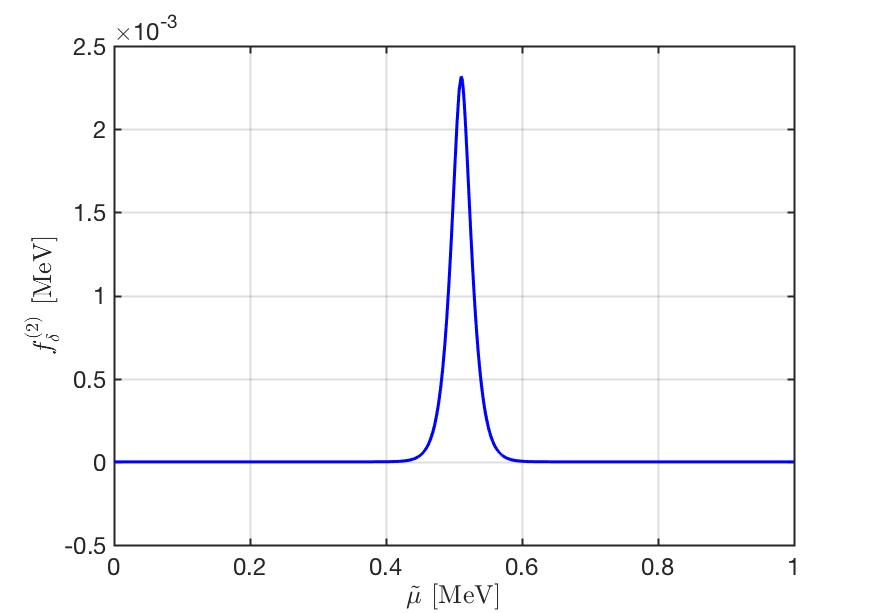
\includegraphics[width=0.9\textwidth]{./plot/f_delta_checking}
\caption{We plot the function$f^{(2)}_\delta$ as a function $E_f$ and we found that the function $f^{(2)}_\delta(E)$ also has peaks when the $E_F=m_e$.}
\label{f_delta_checking_graph}
\end{center}
\end{figure}
%~~~~~~~~~~~~~~~~~~~~~~~~~~~~~~~~~~~~~~~~~~~~~~~~~~~~~~~~~~~~~~~~~~~~~~~~~~~~~~~~~~~~~~~~~~~~~~~~~
In summary, the dimensionless integral can be written as
\begin{align}
&\frac{1}{2}\int^\infty_{x_0}dx\,g^\prime(x)\bigg[e^{-|x|}-e^{-|x_0|}+2\ln\left(\frac{1+e^{-|x_0|}}{1+e^{-|x|}}\right)\bigg]\\
&=\Theta(-x_0)\,\frac{1}{2}\int^{|x_0|}_0dx\,\bigg(g^\prime(x)+g^\prime(-x)\bigg)\bigg[e^{-x}-e^{-|x_0|}+2\ln\left(\frac{1+e^{-|x_0|}}{1+e^{-x}}\right)\bigg]\\&+\frac{1}{2}\int^\infty_{|x_0|}dx\,g^\prime(x)\bigg[e^{-x}-e^{-|x_0|}+2\ln\left(\frac{1+e^{-|x_0|}}{1+e^{-x}}\right)\bigg],
\end{align}
where the $1st$ integral only exist when the Fermi energy $E_F>m_e$ and given function $g^\prime(x)$ is even function. Otherwise we only have the Boltzmann integral.

%%%%%%%%%%%%%%%%%%%%%%%%%%%%%%%%%%%%%%%%%%%%%%%%%%%%%%%%%%%%%%%%%
\subsection{The finite mass integral of $f_\delta(E)$ and $f^{(2)}_\delta(E)$}
In general, the integral that is important for us is the difference between Eq.(\ref{Integral001}) and Eq.(\ref{Integral002}). We have
\begin{align}
\int^{\infty}_{m_e}\,dE\left(g(E)\,f_\delta(E)-g^\prime(E)\,f^{(2)}_\delta(E)\right).
\end{align}
With the variable $x=(E-E_F)/T$ the dimensionless integral can be written as
\begin{align}
\int^{\infty}_{x_0}\,dx\left(g(x)\,f_\delta(x)-g^\prime(x)\,f^{(2)}_\delta(x)\right),
\end{align}
where the parameter $x_0=(m_e-E_F)/T$. To calculate the integral we need to consider the case as follows
\begin{itemize}
  \item For the case: $x_0>0$, i.e., $m_e>E_F$. We have
  \begin{align}
  \int^{\infty}_{x_0}\,dx\left(g(x)\,f_\delta(x)-g^\prime(x)\,f^{(2)}_\delta(x)\right)=\frac{1}{2}\bigg[&\int^\infty_{x_0}dx\left(g(x)-g^\prime(x)\right)\,e^{-x}+\int^{\infty}_{x_0}dxg^\prime(x)\,e^{-x_0}-2\int^\infty_{x_0}dx\ln\left(\frac{1+e^{-x_0}}{1+e^{-x}}\right)\bigg].
  \end{align}
  \item For the case: $x_0<0$, i.e., $m_e<E_F$. We obtain
  \begin{align}
  &\int^{\infty}_{x_0}\,dx\left(g(x)\,f_\delta(x)-g^\prime(x)\,f^{(2)}_\delta(x)\right)\notag\\
  &=\frac{1}{2}\int^{|x_0|}_0dx\bigg\{\bigg[(g(x)+g(-x))-(g^\prime(x)+g^\prime(-x))\bigg]e^{-x}+\bigg(g^\prime(x)+g^\prime(-x)\bigg)e^{-|x_0|}-2\bigg(g^\prime(x)+g^\prime(-x)\bigg)\ln\left(\frac{1+e^{-|x_0|}}{1+e^{-x}}\right)\bigg\}\notag\\
  &+\frac{1}{2}\int^\infty_{|x_0|}dx\bigg\{\bigg[g(x)-g^\prime(x)\bigg]\,e^{-x}+g^\prime(x)\,e^{-|x_0|}-2\,g^\prime(x)\ln\left(\frac{1+e^{-|x_0|}}{1+e^{-x}}\right)\bigg\}
  \end{align}
\end{itemize}
In summary, the dimensionless integral can be written as
\begin{align}
&\int^{\infty}_{x_0}\,dx\left(g(x)\,f_\delta(x)-g^\prime(x)\,f^{(2)}_\delta(x)\right)\\
&=\Theta(-x_0)\,\frac{1}{2}\int^{|x_0|}_0dx\bigg\{\bigg[(g(x)+g(-x))-(g^\prime(x)+g^\prime(-x))\bigg]e^{-x}+\bigg(g^\prime(x)+g^\prime(-x)\bigg)\left[e^{-|x_0|}-2\ln\left(\frac{1+e^{-|x_0|}}{1+e^{-x}}\right)\right]\bigg\}\notag\\
  &+\frac{1}{2}\int^\infty_{|x_0|}dx\bigg\{\bigg[g(x)-g^\prime(x)\bigg]\,e^{-x}+g^\prime(x)\,e^{-|x_0|}-2\,g^\prime(x)\ln\left(\frac{1+e^{-|x_0|}}{1+e^{-x}}\right)\bigg\}.
\end{align}
The $1st$ integral only exist when the $x_0<0$, i.e., $m_e<E_F$. We believe that the $1st$ integral capture the essence of the nonequilibrium property.

%%%%%%%%%%%%%%%%%%%%%%%%%%%%%%%%%%%%%%%%%%%%%%%%%%%%%%%%%%%%%%%%%

\section{Appendix: calculation of $f^{(2)}_\delta(E)$ in detail}
The quantity $f^{(2)}_\delta(E)$ can be written as
\begin{align}
\label{f_delta}
f^{(2)}_\delta(E)&=\int^{E}_{m_e}\,dE^\prime\,\frac{1}{2}\bigg[\Theta(E_F-E^\prime)\,e^{(E^\prime-E_F)\beta}+\Theta(E^\prime-E_F)\,e^{-(E^\prime-E_F)\beta}\bigg]\,\tanh\bigg[\frac{E^\prime-E_F}{2T}\bigg]\notag\\
&=\int^{E}_{m_e}\,dE^\prime\,\frac{1}{2}\bigg[\Theta(E_F-E^\prime)\,e^{(E^\prime-E_F)\beta}+\Theta(E^\prime-E_F)\,e^{-(E^\prime-E_F)\beta}\bigg]\,\frac{e^{(E^\prime-E_f)/T}-1}{e^{(E^\prime-E_F)/T}+1}\notag\\
&=\frac{1}{2}\int^{E}_{m_e}\,dE^\prime\,\Theta(E_F-E^\prime)\,e^{(E^\prime-E_F)\beta}\frac{e^{(E^\prime-E_f)/T}-1}{e^{(E^\prime-E_F)/T}+1}+\frac{1}{2}\int^{E}_{m_e}\,dE^\prime\,\Theta(E^\prime-E_F)\,e^{-(E^\prime-E_F)\beta}\frac{e^{(E^\prime-E_f)/T}-1}{e^{(E^\prime-E_F)/T}+1}
\end{align}
To calculate the integrals, it is convenient to compare the $E_F$ and $m_e$ first. From Eq.(\ref{f_delta}), the first integral can be written as
\begin{itemize}
\item For $E_F>E>m_e$, we have:
\begin{align}
&\frac{1}{2}\int^{E}_{m_e}\,dE^\prime\,\Theta(E_F-E^\prime)\,e^{(E^\prime-E_F)\beta}\frac{e^{(E^\prime-E_f)/T}-1}{e^{(E^\prime-E_F)/T}+1}\\&=\frac{1}{2}\int^{E}_{m_e}\,dE^\prime\,e^{(E^\prime-E_F)\beta}\frac{e^{(E^\prime-E_f)/T}-1}{e^{(E^\prime-E_F)/T}+1}=\frac{T}{2}\bigg[e^{-(E_F-E)/T} -e^{-(E_F-m_e)/T} + 2\ln{\left(\frac{1+e^{-(E_F-m_e)/T}}{1+e^{-(E_F-E)/T}}\right)}\bigg]
\end{align}
  \item For $E>E_F>m_e$, we have:
\begin{align}
&\frac{1}{2}\int^{E}_{m_e}\,dE^\prime\,\Theta(E_F-E^\prime)\,e^{(E^\prime-E_F)\beta}\frac{e^{(E^\prime-E_f)/T}-1}{e^{(E^\prime-E_F)/T}+1}\\&=\frac{1}{2}\int^{E_F}_{m_e}\,dE^\prime\,e^{(E^\prime-E_F)\beta}\frac{e^{(E^\prime-E_f)/T}-1}{e^{(E^\prime-E_F)/T}+1}=\frac{T}{2}\bigg[(1-\ln4)-e^{-(E_F-m_e)/T} + 2\ln{\left(1+e^{-(E_F-m_e)/T}\right)}\bigg]
\end{align}
  \item For $E>m_e>E_F$, we have:
\begin{align}
\frac{1}{2}\int^{E}_{m_e}\,dE^\prime\,\Theta(E_F-E^\prime)\,e^{(E^\prime-E_F)\beta}\frac{e^{(E^\prime-E_f)/T}-1}{e^{(E^\prime-E_F)/T}+1}=0
\end{align}
\end{itemize}
On the other hand, the second integral in Eq.(\ref{f_delta}) can be written as
\begin{itemize}
 \item For $E_F>E>m_e$, we have:
\begin{align}
&\frac{1}{2}\int^{E}_{m_e}\,dE^\prime\,\Theta(E^\prime-E_F)\,e^{-(E^\prime-E_F)\beta}\frac{e^{(E^\prime-E_f)/T}-1}{e^{(E^\prime-E_F)/T}+1}=0
\end{align}
  \item For $E>E_F>m_e$, we have:
\begin{align}
&\frac{1}{2}\int^{E}_{m_e}\,dE^\prime\,\Theta(E^\prime-E_F)\,e^{-(E^\prime-E_F)\beta}\frac{e^{(E^\prime-E_f)/T}-1}{e^{(E^\prime-E_F)/T}+1}\\
&=\frac{1}{2}\int^{E}_{E_F}\,dE^\prime\,e^{-(E^\prime-E_F)\beta}\frac{e^{(E^\prime-E_f)/T}-1}{e^{(E^\prime-E_F)/T}+1}=\frac{T}{2}\bigg[(-1+\ln4)+e^{(E_F-E)/T} -2\ln{\left(1+e^{(E_F-E)/T}\right)}\bigg]
\end{align}
  \item For $E>m_e>E_F$, we have:
\begin{align}
&\frac{1}{2}\int^{E}_{m_e}\,dE^\prime\,\Theta(E^\prime-E_F)\,e^{-(E^\prime-E_F)\beta}\frac{e^{(E^\prime-E_f)/T}-1}{e^{(E^\prime-E_F)/T}+1}\\
&=\frac{1}{2}\int^{E}_{m_e}\,dE^\prime\,e^{-(E^\prime-E_F)\beta}\frac{e^{(E^\prime-E_f)/T}-1}{e^{(E^\prime-E_F)/T}+1}=\frac{T}{2}\bigg[e^{(E_F-E)/T}-e^{(E_F-m_e)/T}+2\ln{\left(\frac{1+e^{(E_F-m_e)/T}}{1+e^{(E_F-E)/T}}\right)}\bigg].
\end{align}
\end{itemize}
In this case, the function  $f^{(2)}_\delta$ can be written as
\begin{align}
f^{(2)}_\delta(E)=\left\{\begin{array}{c}
\frac{T}{2}\left[e^{-(E_F-E)/T}-e^{-(E_F-m_e)/T}+2\ln{\left(\frac{1+e^{-(E_F-m_e)/T}}{1+e^{-(E_F-E)/T}}\right)}\right],\,\,\,\mathrm{for}\,\,\,\,E_F>E>m_e \\ 
\frac{T}{2}\left[e^{(E_F-E)/T}-e^{-(E_F-m_e)/T}+2\ln{\left(\frac{1+e^{-(E_F-m_e)/T}}{1+e^{(E_F-E)/T}}\right)}\right],\,\,\,\,\,\,\,\,\mathrm{for}\,\,\,\,E>E_F>m_e \\
\frac{T}{2}\left[e^{(E_F-E)/T}-e^{(E_F-m_e)/T}+2\ln{\left(\frac{1+e^{(E_F-m_e)/T}}{1+e^{(E_F-E)/T}}\right)}\right],\,\,\,\,\,\,\,\,\mathrm{for}\,\,\,\,E>m_e>E_F
\end{array}\right.
\end{align}
In general, it can be written as
\begin{align}
f^{(2)}_\delta(E)=\frac{T}{2}\left[e^{-|E_F-E|/T}-e^{-|E_F-m_e|/T}+2\ln{\left(\frac{1+e^{-|E_F-m_e|/T}}{1+e^{-|E_F-E|/T}}\right)}\right].
\end{align}
In Fig.(\ref{f_delta_checking}) we plot the function $f^{(2)}_\delta$ as a function of Fermi-energy $E$ for the case $E_F>m_e$ . We found that the behavior of $f^{(2)}_\delta$  is like delta function with peak at $E=E_F$. 
%~~~~~~~Figure~~~~~~~~~~~~~~~~~~~~~~~~~~~~~~~~~~~~~~~~~~~~~~~~~~~~~~~~~~~~~~~~~~~~~~~~~~~~~~~~~~~~~
\begin{figure}[t]
\begin{center}
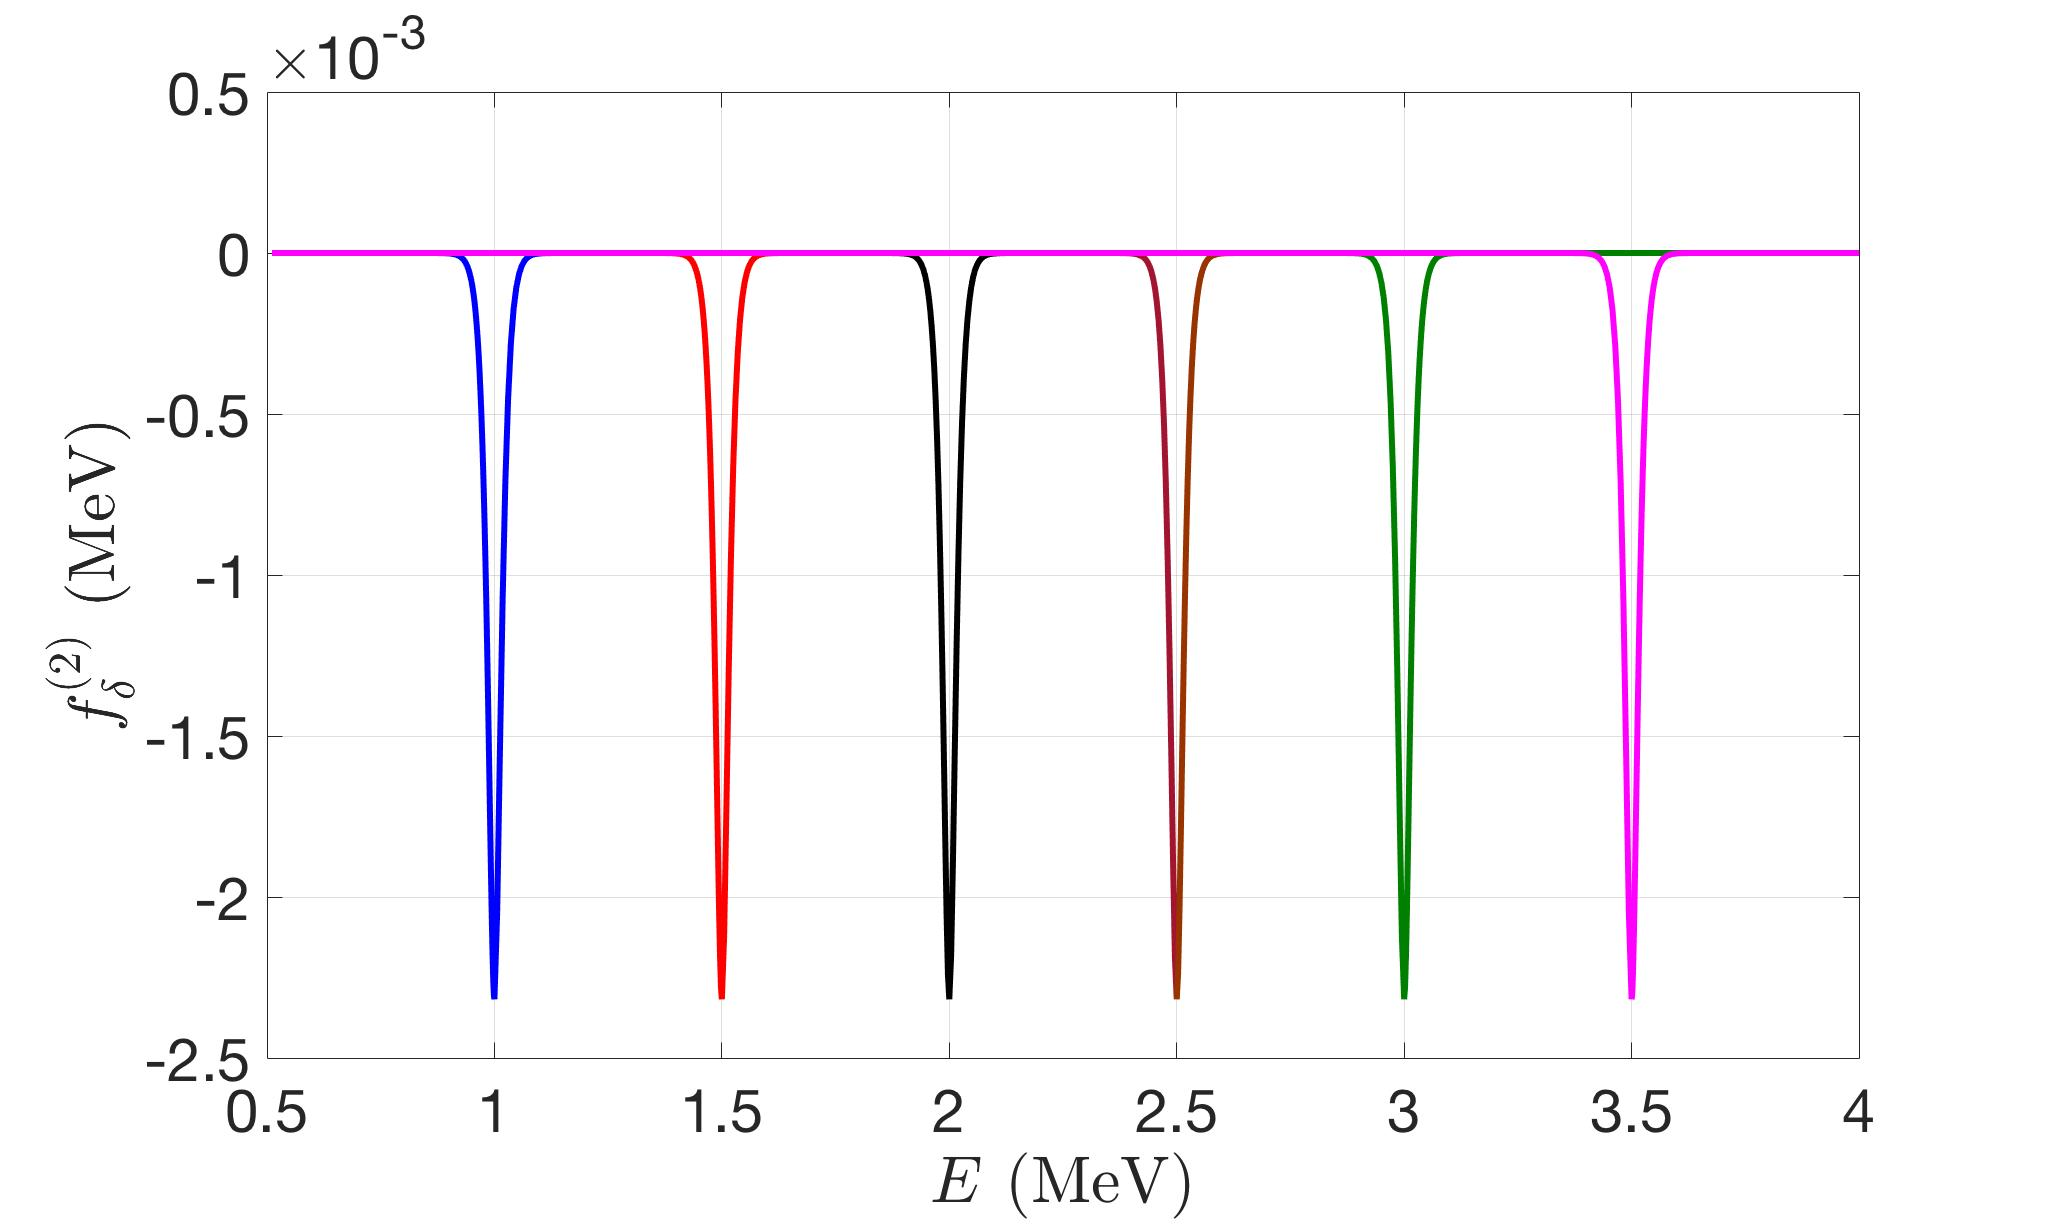
\includegraphics[width=0.9\textwidth]{./plot/f_delta_checking2}
\caption{We plot the function $f^{(2)}_\delta$ as a function of energy $E$ with $T=0.012\,\mathrm{MeV}$. We found that the behavier of $f^{(2)}_\delta$  is like delta function with peak at $E=E_F$. We have  $E_F=1.0\,\mathrm{MeV}, 1.5\,\mathrm{MeV}, 2.0\,\mathrm{MeV},2.5\,\mathrm{MeV}, 3.0\,\mathrm{MeV}, 3.5\,\mathrm{MeV}$.}
\label{f_delta_checking}
\end{center}
\end{figure}
%~~~~~~~~~~~~~~~~~~~~~~~~~~~~~~~~~~~~~~~~~~~~~~~~~~~~~~~~~~~~~~~~~~~~~~~~~~~~~~~~~~~~~~~~~~~~~~~

%\begin{align}
%N_e^{cold}=\frac{g_eV}{2\pi^2}\int^{E_F}_{m_e}{dE}E\sqrt{E^2-m^2_e}=\frac{g_eV\,(E_F^2-m_e^2)^{3/2}}{6\pi^2}
%\end{align}
%then the the number of electron in early universe can be written as
%\begin{align}
%N_e=N_e^{cold}&-\frac{g_eV}{2\pi^2}\int^{E_F}_{m_e}{dE}\frac{E\sqrt{E^2-m^2_e}}{2}\,\bigg[1-\tanh\bigg(\frac{E-E_F}{2T}\bigg)\bigg]\,e^{(E-E_F)/T}\notag\\&+\frac{g_eV}{2\pi^2}\int^{\infty}_{E_F}\,{dE}\frac{E\sqrt{E^2-m^2_e}}{2}\,\bigg[1+\tanh\bigg(\frac{E-E_F}{2T}\bigg)\bigg]\,e^{-(E-E_F)/T}.
%\end{align}

%%%%%%%%%%%%%%%%%%%%%%%%%%%%%%%%%%%%%%%%%%%%%%%%%%%%%%%%%%%%%%

\begin{thebibliography}{99}

\bibitem{Kuznetsova:2008jt}
I.~Kuznetsova, D.~Habs and J.~Rafelski,
``Pion and muon production in e-, e+, gamma plasma,''
Phys.\ Rev.\ D \textbf{78}, 014027 (2008)
doi:10.1103/PhysRevD.78.014027
[arXiv:0803.1588 [hep-ph]].

%\bibitem{Mukhanov:2012mu}
%Viatcheslav~Mukhanov,~"Physical Foundations of Cosmology
 
%\bibitem{Tanabashi:2018oca} 
%M.~Tanabashi {\it et al.} [Particle Data Group],
%``Review of Particle Physics,''
%Phys.\ Rev.\ D {\bf 98}, no. 3, 030001 (2018).
%doi:10.1103/PhysRevD.98.030001

%\bibitem{Letessier:2002gp} 
%J.~Letessier and J.~Rafelski,
%``Hadrons and quark - gluon plasma,''
%Camb.\ Monogr.\ Part.\ Phys.\ Nucl.\ Phys.\ Cosmol.\ {\bf 18} (2002).

%\bibitem{Giunti:2007gi}
%Carlo~Giunti,~"Fundamentals of Neutrino Physics and Astrophysics

 \end{thebibliography}
%%%%%%%%%%%%%%%%%%%%%%%%%%%%%%%%%%%%%%%%%%%%%%%%%%%%%%%%%%%%%%
\end{document} 
